\documentclass[11pt,a4paper]{article}

\usepackage{amsmath}
\usepackage{amsfonts}
\usepackage{geometry}
\usepackage{graphicx}
\usepackage{fancyhdr}
\usepackage{setspace}
\usepackage{amssymb}
\usepackage{booktabs}
\usepackage{enumitem}
\usepackage{multirow}
\usepackage{titlesec}
\usepackage{caption}
\usepackage{subcaption}
\usepackage{float}
\usepackage{tabularx}
\usepackage{braket}
\usepackage{listings}

\usepackage{algorithm, algpseudocode}
\usepackage{algorithm}
\usepackage{algpseudocode}

\setcounter{secnumdepth}{4}

% set table of content depth
\setcounter{tocdepth}{3} 
\usepackage[titles]{tocloft}

% set spacing 
\setlength{\cftbeforesecskip}{10pt}

% Page layout settings
\geometry{
  a4paper,
  left=20mm,
  right=20mm,
  top=25mm,
  bottom=25mm
}

\usepackage{biblatex}
\addbibresource{Project_Report_References.bib}

%%%%%%%%%%%%%%%%%%%%%%%%%%%%%%%%%%%%%%%%%%%%%%%%%%%%%%%%%%%%%%%%%
%%%%%%%%%%%%%%%%%%%%%%%%%%%%%%%%%%%%%%%%%%%%%%%%%%%%%%%%%%%%%%%%%
\begin{document}
\singlespacing % Set the document to single line spacing
\thispagestyle{empty} % Remove page number for the cover page

\begin{center}
{\bf \LARGE Approaches to Noise Resilient Quantum Circuit Design}\\[0.5cm]
  \textbf{Christian Wood} \\[0.2cm]
  \textbf{Student ID:} 710018541 \\[1cm]
\end{center}

\section*{Abstract}
\noindent 
One of the key challenges in quantum computing is designing quantum circuits, a task made difficult by their probabilistic behaviour and counter-intuitive nature. Various automated techniques have been proposed, with genetic algorithms emerging as a popular method. In the current NISQ era, quantum noise poses a serious obstacle by introducing significant computational errors. By leveraging multi-objective evolutionary algorithms (MOEAs), our approach not only automates circuit design but also includes additional criteria to enhance performance under realistic noisy conditions. We present an MOEA with an a priori decision maker that adapts to the design of arbitrary circuits along with a novel circuit representation scheme. We demonstrate the method’s effectiveness by applying it to the 2 and 3-qubit Quantum Fourier Transform (QFT), showing that the approach evolves circuits that not only replicate the desired circuit's behaviour, but also outperform traditional circuits under noisy conditions.

\newpage
\thispagestyle{empty} 
\section*{Declaration}
I acknowledge the following uses of GenAI tools in this assessment: 

\begin{itemize}[label={\ $\square$\ }, leftmargin=*]
 \item I have used GenAI tools to:
 \begin{itemize}[label={\ $\square$\ }, leftmargin=*]
  \item develop ideas.
  \item assist with research or gathering information.
  \item help me understand key theories and concepts.
  \item identify trends and themes as part of my data analysis.
  \item suggest a plan or structure for my assessment.
  \item give me feedback on a draft.
  \item generate images, figures or diagrams.
  \item proofread and correct grammar or spelling errors.
  \item generate citations or references.
  \item Other: [please specify]
  \item[]
 \end{itemize}
 \item I have not used any GenAI tools in preparing this assessment.
\end{itemize}

\bigskip
I declare that I have referenced all use of GenAI outputs within my assessment in line with the University referencing guidelines.

\vspace{1em}
I certify that all material in this dissertation which is not my own has been identified. 

\vspace{5em}
{\bf\noindent Signature:} \hrulefill
\newpage

% Table of Contents
\tableofcontents 
\thispagestyle{empty} 
\newpage 

% Reset page numbering for main report
\clearpage
\pagenumbering{arabic} 

%%%%%%%%%%%%%%%%%%%%%%%%%%%%%%%%%%%%%%%%%%%%%%%%%%%%%%%%%%%%%%%%%
%
%  Introduction
%
%%%%%%%%%%%%%%%%%%%%%%%%%%%%%%%%%%%%%%%%%%%%%%%%%%%%%%%%%%%%%%%%%
\section{Introduction}
Quantum computing represents a fundamental shift in computational paradigms, harnessing the principles of quantum mechanics to perform operations that are infeasible on classical machines. Unlike classical bits, which are strictly binary, quantum bits, known as qubits, exploit superposition \cite{Gudder1970ASP}, allowing them to exist in a linear combination of both $\ket{0}$ and $\ket{1}$ states simultaneously. Alongside this, the phenomenon of quantum entanglement \cite{horodecki2009quantum} permits correlations between qubits that transcend classical limits, enabling quantum systems to explore vast computational spaces in parallel.\newline

This inherent parallelism underpins quantum computing’s potential to offer exponential or quadratic speedups for a variety of computational problems that are otherwise intractable on classical architectures. Shor’s algorithm \cite{Shor365700}, for instance, enables exponential acceleration in integer factorisation, posing a credible threat to classical cryptographic schemes. Similarly, Grover’s algorithm \cite{Khanal2021QuantumML} achieves a quadratic improvement in unstructured search problems. These theoretical milestones showcase quantum computing’s transformative potential across fields including cryptography, optimisation, chemistry, and materials science.\newline

However, the realisation of practical quantum algorithms remains constrained by the limitations of contemporary quantum hardware. We are currently situated in the so-called Noisy Intermediate-Scale Quantum (NISQ) era \cite{Preskill2018QuantumCI}, characterised by devices with tens to a few thousand qubits and plagued by noise, decoherence, and limited connectivity. Quantum operations, especially multi-qubit gates, are subject to high error rates, and circuit depth correlates directly with the likelihood of computation failure \cite{Clerk2008IntroductionTQ}. Compounding these hardware limitations is the intrinsic complexity of quantum circuit design. Unlike classical circuit construction, which is guided by well-established logic frameworks, quantum circuits must obey strict unitary constraints, preserve reversibility, and be robust to decoherence, rendering manual design both difficult and unintuitive. This motivates the need for automated circuit synthesis techniques that can navigate large, complex design spaces.\newline

One promising strategy is the use of Evolutionary Algorithms (EAs) \cite{Lukac2002EvolvingQC}, a class of bio-inspired metaheuristics capable of discovering solutions through principles of selection, variation, and inheritance. Multi-Objective Evolutionary Algorithms (MOEAs) \cite{moein} extend this paradigm by simultaneously optimising competing objectives such as fidelity and circuit depth. This allows for the discovery of quantum circuits that are both correct and better suited to noisy, imperfect hardware.\newline

In this work, we propose a novel MOEA-based framework for quantum circuit design that employs a layer-based encoding scheme to support concurrent gate execution. The framework integrates custom genetic operators and a scalarised fitness function that balances fidelity to ideal outputs, performance under realistic noise models, and circuit depth. This methodology enables efficient search for quantum circuits that are both structurally compact and noise-resilient.\newline

To demonstrate its efficacy, we apply the framework to the Quantum Fourier Transform (QFT) \cite{Jozsa1997QuantumAA}, a canonical subroutine in many quantum algorithms including Shor’s and quantum phase estimation. The QFT’s regular structure and sensitivity to noise make it a suitable benchmark for testing automated design approaches. We present results for evolved QFT implementations across both 2- and 3-qubit configurations, showing that our evolved circuits outperform textbook designs under noisy conditions.\newline

The remainder of this dissertation is structured as follows: Section~\ref{sec:background} expands on the background and challenges in NISQ circuit design. Section~\ref{sec:design} outlines the design of our genetic algorithm. Section~\ref{sec:experimental} details the experimental setup, followed by results and evaluations in Section~\ref{sec:results}. Section~\ref{sec:analysis} provides critical analysis, and Section~\ref{sec:conclusion} concludes with future directions.

%%%%%%%%%%%%%%%%%%%%%%%%%%%%%%%%%%%%%%%%%%%%%%%%%%%%%%%%%%%%%%%%%
%
%  Background and Research Goals
%
%%%%%%%%%%%%%%%%%%%%%%%%%%%%%%%%%%%%%%%%%%%%%%%%%%%%%%%%%%%%%%%%%
\section{Background and Research Goals} \label{sec:background}
\subsection{Background}
\subsubsection*{Quantum Noise and Circuit Fidelity}
Quantum circuits operating on NISQ-era hardware are highly susceptible to various types of noise, including amplitude damping, dephasing, and depolarisation \cite{Clerk2008IntroductionTQ}. These effects are particularly severe in multi-qubit gates such as CNOTs, which exhibit significantly higher error rates than single-qubit operations. Circuit depth strongly correlates with the accumulation of noise, making depth minimisation a crucial goal for practical algorithm deployment.\newline

Simulators such as Qiskit Aer allow for realistic modelling of hardware-specific noise profiles, including composite error channels that combine depolarisation with amplitude and phase damping. This capability enables developers to evaluate candidate circuits in noisy conditions prior to execution on physical devices.

\subsubsection*{Motivation for Evolutionary Approaches}
These challenges, noise, connectivity, and circuit complexity, create a multi-faceted optimisation problem. Evolutionary Algorithms (EAs) are well-suited to this setting due to their ability to explore high-dimensional, discontinuous search spaces without the need for gradient information. When extended to Multi-Objective Evolutionary Algorithms (MOEAs), they further support trade-offs between competing goals, such as fidelity and circuit depth \cite{moein, Zhou2011MultiobjectiveEA}.\newline

Importantly, the representation of candidate solutions plays a crucial role in evolutionary search. Serial encodings lack support for parallel gate execution, making them ill-suited to NISQ constraints. By contrast, layer-based representations naturally support concurrent gate application and enable more meaningful variation through genetic operations.

\subsection{Why Quantum Fourier Transform (QFT)?}
The Quantum Fourier Transform (QFT) was selected as the target benchmark for this work due to its well-defined mathematical structure, practical importance in quantum algorithms, and the non-trivial challenges it poses for circuit synthesis. As a core subroutine in algorithms such as Shor’s factoring algorithm and quantum phase estimation, the QFT is a canonical example of a structured quantum computation with clear correctness criteria and known optimal implementations.\newline

Unlike trivial or randomly generated unitaries, the QFT allows for meaningful comparison between evolved circuits and textbook designs, both in terms of fidelity and gate-level structure. Furthermore, it strikes a balance between complexity and tractability. Small-scale QFT circuits (2 to 3 qubits) are sufficiently expressive to expose optimisation challenges, such as depth minimisation, entanglement management, and noise sensitivity, while remaining computationally feasible for repeated evaluation during evolution.\newline

From an evolutionary optimisation perspective, the QFT's layered, recursive structure makes it a compelling target: its solution space is rich with locally optimal variants that differ in depth, entanglement structure, and parameterisation. This opens up avenues for innovation beyond textbook templates, providing an ideal testbed for evaluating the effectiveness of custom genetic operators in balancing competing constraints such as noise resilience and circuit complexity.

\subsection{Research Objectives}\label{sec:objectives}
Building upon this background, the primary aim of this dissertation is to investigate the effectiveness of a bespoke MOEA framework for quantum circuit synthesis on NISQ hardware. The specific research objectives are as follows:

\begin{enumerate}
    \item \textbf{Design an EA capable of Reproducing Ideal Circuit Behaviour:} Develop an EA with our proposed circuit encoding scheme and associated genetic operators with a fitness function aimed at replicating ideal circuit behaviour.
    
    \item \textbf{Implement an MOEA Integrating Noise Remediating Techniques:} Combine ideal state fidelity, noisy output fidelity (via simulation), and depth penalties into a single evaluation metric that promotes efficient, noise-resilient designs.
    
    \item \textbf{Benchmark Performance against the Traditional QFT Circuit:} pply the framework to 2- and 3-qubit Quantum Fourier Transform circuits and compare evolved variants against textbook implementations in both noiseless and noisy environments.
\end{enumerate}

Through these objectives, this work seeks to demonstrate the viability of MOEA-guided quantum circuit design as a tool for bridging the gap between theoretical algorithm design and practical execution on near-term quantum hardware.

%%%%%%%%%%%%%%%%%%%%%%%%%%%%%%%%%%%%%%%%%%%%%%%%%%%%%%%%%%%%%%%%%
%
%  Genetic Algorithm Design
%
%%%%%%%%%%%%%%%%%%%%%%%%%%%%%%%%%%%%%%%%%%%%%%%%%%%%%%%%%%%%%%%%%
\section{Genetic Algorithm Design}\label{sec:design}
\subsection{Circuit Representation}
A central challenge in applying evolutionary algorithms to quantum circuit design lies in creating a representation that is both expressive enough to capture complex quantum behaviour, and structured enough to permit efficient manipulation through genetic operators. This work adopts a layer-based representation scheme, inspired by the block-based encodings used in previous literature~\cite{Lukac2002EvolvingQC}, with enhancements designed to support noise-aware optimisation on NISQ devices.\newline

Each circuit is represented by a chromosome using an ordered list of layers, where each layer corresponds to a discrete timestep. A layer is a list of gate specification strings, one per qubit, indicating the operation (if any) applied to that qubit during that timestep. Single-, two-, and three-qubit gates are supported, including parametrised variants. Gates applied within the same layer must act on disjoint sets of qubits, enabling concurrent execution and directly influencing the circuit’s effective depth.

\subsubsection*{Gate Specifications} Each gate is encoded as a string using the format gate(args), where args may include control qubit indices and rotation parameters. Partner qubits in multi-qubit gates are marked with a special symbol "-", while idle qubits are annotated with a "w" (barrier). Table~\ref{tab:gateset} summarises the full gate set used in this work, including arities, parameters, and descriptions.

\begin{table}[H]
    \centering
    \begin{tabular}{llll}
        \toprule
        \textbf{Gate} & \textbf{Qubit Arity} & \textbf{Parameters} & \textbf{Description} \\
        \midrule
        x, y, z, h, s, sdg, t, tdg & 1 & None & Basic single-qubit gates \\
        rx, ry, rz & 1 & $\theta$ & Rotation around X, Y, or Z axis \\
        cx, cy, cz & 2 & control & Controlled Pauli operations \\
        swap & 2 & None & Swap operation \\
        crx, cry, crz, cp & 2 & control, $\theta$ & Controlled rotations or phase \\
        rxx, ryy, rzz & 2 & $\theta$ & Two-qubit interaction gates \\
        ccx & 3 & control$_1$, control$_2$ & Toffoli gate \\
        cswap & 3 & control, target$_1$, target$_2$ & Controlled-SWAP gate \\
        - & 0 & None & Control marker (non-target) \\
        w & 0 & None & No operation \\
        \bottomrule
    \end{tabular}
    \caption{Summary of the gate set used in the evolutionary framework.}
    \label{tab:gateset}
\end{table}

\subsubsection*{Example Chromosome} Figure~\ref{fig:chromosome_list} presents a representative chromosome for a 3-qubit system, showing the gate specification strings for each layer. Figure~\ref{fig:chromosome_matrix} shows a more intuitive visualisation of this with each inner list in the 2D array running vertically. ~\ref{fig:chromosome_circuit} shows the interpreted quantum circuit resulting from this representation.

\begin{figure}[H]
    \centering

    % Subfigure 1 - List Representation
    \begin{subfigure}[b]{0.9\textwidth}
        \centering
        \texttt{[['h', 'w', 'w'], ['cp(0,1,1.5707)', '-', 'w'], ['cp(0,2,0.7853)', 'w', '-'], ['w', 'h', 'w'], 
        ['w', 'cp(1,2,1.5707)', '-'], ['w', 'w', 'h'], ['swap(0,2)', 'w', '-']]}
        \caption{Chromosome List Representation}
        \label{fig:chromosome_list}
    \end{subfigure}

    \vspace{1em}

    % Subfigure 2 - Tabular Matrix
    \begin{subfigure}[b]{0.65\textwidth}
        \centering
        \small
        \begin{tabular}{l | c c c c c c c}
            \toprule
            Qubit 0 & h & p(1,1.5707) & cp(2,0.7853) & w & w & w & swap(2) \\
            \midrule
            Qubit 1 & w & - & w & h & cp(2,1.5707) & w & w \\
            \midrule
            Qubit 2 & w & w & - & w & - & h & - \\
            \bottomrule
        \end{tabular}
        \caption{Matrix Interpretation}
        \label{fig:chromosome_matrix}
    \end{subfigure}

    \vspace{1em}

    % Subfigure 3 - Circuit Diagram
    \begin{subfigure}[b]{0.6\textwidth}
        \centering
        \includegraphics[width=\textwidth]{Images/qft_traditional.png}
        \caption{Interpreted Quantum Circuit}
        \label{fig:chromosome_circuit}
    \end{subfigure}

    \caption{Different representations of a quantum chromosome: raw list (a), gate matrix (b), and resulting circuit (c).}
    \label{fig:chromosome_representations}
\end{figure}\newpage

\subsubsection*{Layer Construction}
The creation of a new layer is governed by a stochastic process implemented in the create\_new\_layer() function. Each qubit position is assigned a gate drawn from a weighted distribution, where the no-op gate ("w") has a fixed probability, and the remainder is split among valid single-, double-, and triple-qubit gates. If a multi-qubit gate is selected, the appropriate control qubit(s) are assigned using free indices in the layer, and their positions are marked with "-". This ensures no gate overlaps occur within a single timestep, preserving physical validity.

\subsubsection*{Parsing and Circuit Construction}
Once the chromosome is fully constructed, the gate specification strings are parsed using parse\_gate\_spec(), which extracts the gate name and arguments. A mapping table implemented in build\_gate\_map() links each gate to a corresponding Qiskit function. The final circuit is assembled via get\_circuits(), which processes the chromosome layer-by-layer and applies each gate to a growing QuantumCircuit object. All operations in a layer are executed in parallel.

\subsubsection*{Advantages}
\begin{itemize}
    \item \textbf{Parallelism-aware:} Enables concurrent gate execution, reducing circuit depth and noise accumulation.
    \item \textbf{Genetically robust:} Supports meaningful crossover and mutation at the layer level without violating circuit integrity.
    \item \textbf{Hardware-aligned:} Compatible with transpiler constraints and hardware scheduling on real quantum devices.
    \item \textbf{Semantically expressive:} Encodes both gate type and qubit roles compactly, including support for parametrised operations.
\end{itemize}

In summary, this layer-based circuit representation enables both expressive modelling and efficient evolution of quantum circuits under noisy constraints. Its compatibility with hardware and genetic operators makes it a core component of the evolutionary framework presented in this work.

\subsection{Genetic Operators}
The evolutionary process in this work is driven by a suite of custom genetic operators tailored to the layered circuit representation. These operators explore the solution space and guide the search towards functionally correct, low‐depth, noise‐resilient quantum circuits. The standard three‐stage paradigm of selection, crossover and mutation is retained, but each stage has been adapted to the particular constraints and opportunities of NISQ‐era quantum circuit design.

\subsubsection*{Parent Selection}
Parent selection determines which individuals contribute genetic material to the next generation, directly affecting both convergence speed and population diversity. In our experiments we systematically compared several well‐known strategies:

\begin{itemize}
    \item \textbf{Random selection} picks individuals uniformly at random, guaranteeing maximal exploration but offering no preference for higher‐fitness solutions. Early trials showed that this approach led to erratic progress and slow convergence, as good solutions were no more likely to reproduce than poor ones.
    \item \textbf{Fitness‐proportionate (roulette‐wheel) selection} assigns reproduction probability proportional to an individual’s fitness. While this method rewards better solutions, it suffered from severe fitness scaling issues: when a few individuals achieved markedly higher fitness, they came to dominate reproduction, leading to premature convergence and loss of diversity.
    \item \textbf{Tournament selection} samples a small subset of the population and selects the best among them. Varying the tournament size allowed us to tune selection pressure, but the stochastic nature of sampling introduced high variance in convergence rates, especially for small populations. An elitist variant, guaranteeing the best of each tournament advanced unconditionally, improved stability but still exhibited occasional regressions.
\end{itemize}

After extensive testing, \textbf{rank‐based selection with elitism} emerged as the most effective. In this method, all individuals are sorted by fitness and assigned ranks from 1 (lowest) to $N$ (highest). Selection probabilities increase linearly with rank, which normalises the effect of fitness differences and prevents outliers from overwhelming the gene pool. Concurrently, the top one‐third of the population is preserved unchanged into the next generation (elitism). This hybrid strategy ensures that superior solutions are never lost to stochastic fluctuations, while still permitting lower‐fitness individuals to contribute, thereby sustaining exploratory dynamics. Over dozens of runs, this approach delivered the fastest and most reliable improvements in circuit fidelity.

\subsubsection*{Crossover}
Crossover recombines structural information from two parent chromosomes to form offspring. Given the temporal and parallel nature of layer‐based circuits, we implemented a \textbf{single‐point, layer‐wise crossover}. Two parents are selected via the rank‐based mechanism described above, and a crossover point is chosen uniformly at random between valid layer indices. The child inherits all layers up to this point from Parent A, and the remaining layers from Parent B, preserving gate order and inter‐layer dependencies.

% Parent Chromosomes Figure
\begin{figure}[H]
  \centering
  \begin{subtable}{0.45\textwidth}
    \small
    \begin{tabularx}{\textwidth}{c|*{4}{>{\centering\arraybackslash}X}}
      \toprule
      \multicolumn{5}{c}{\textbf{Parent A}} \\
      \midrule
      Qubit & L0 & L1 & L2 & L3\\
      \midrule
      Qubit 0 & h & cp(1,1.57) & cp(2,0.78) & w \\
      Qubit 1 & w & - & w & h \\
      Qubit 2 & w & w & - & w \\
      \bottomrule
    \end{tabularx}
  \end{subtable}
  \hfill
  \begin{subtable}{0.45\textwidth}
    \small
    \begin{tabularx}{\textwidth}{c|*{4}{>{\centering\arraybackslash}X}}
      \toprule
      \multicolumn{5}{c}{\textbf{Parent B}} \\
      \midrule
      Qubit & L0 & L1 & L2 & L3\\
      \midrule
      Qubit 0 & x & h & z & w \\
      Qubit 1 & x & w & cz(1.00) & w \\
      Qubit 2 & w & ry(3.30) & - & h \\
      \bottomrule
    \end{tabularx}
  \end{subtable}
  \caption{Side‐by‐side parent chromosomes}.
  \label{fig:parents_tabularx}
\end{figure}

% Child Chromosomes Figure
\begin{figure}[H]
  \centering
  \begin{subtable}{0.45\textwidth}
    \small
    \caption{Child A (layers 0-2 from Parent A, layer 3 from Parent B)}
    \label{tab:child1}
    \begin{tabularx}{\textwidth}{c|*{4}{>{\centering\arraybackslash}X}}
      \toprule
      \multicolumn{5}{c}{\textbf{Child A}} \\
      \midrule
      Qubit & L0 & L1 & L2 & L3 \\
      \midrule
      Qubit 0 & h & cp(1,1.57) & cp(2,0.78) & w \\
      Qubit 1 & w & – & w & w \\
      Qubit 2 & w & w & – & h \\
      \bottomrule
    \end{tabularx}
  \end{subtable}
  \hfill
  \begin{subtable}{0.45\textwidth}
    \small
    \caption{Child B (layers 0-2 from Parent B, layer 3 from Parent A)}
    \label{tab:child2}
    \begin{tabularx}{\textwidth}{c|*{4}{>{\centering\arraybackslash}X}}
      \toprule
      \multicolumn{5}{c}{\textbf{Child B}} \\
      \midrule
      Qubit & L0 & L1 & L2 & L3 \\
      \midrule
      Qubit 0 & x & h & z & w \\
      Qubit 1 & x & w & cz(1.00) & h \\
      Qubit 2 & w & ry(3.30) & – & w \\
      \bottomrule
    \end{tabularx}
  \end{subtable}
  \caption{Offspring chromosomes produced by single‑point, layer‑wise crossover (crossover point between layers 2 and 3).}
  \label{fig:children_tabularx}
\end{figure}

This crossover operator preserves the temporal integrity of gate sequences while enabling the mixing of high‐performance subcircuits. In practice, the recombination of fidelity‐preserving prefixes with noise‐resistant suffixes often yields offspring that outperform both parents after subsequent mutation.

\subsubsection*{Mutation}
Mutation introduces essential variation into the population, enabling the evolutionary process to escape local optima and discover novel circuit topologies. In our framework, mutation is applied at three hierarchical levels:

\begin{enumerate}
  \item \textbf{Parameter‑level mutation} perturbs the continuous rotation angles of parametrised gates, refining phase relationships.
  \item \textbf{Gate‑level mutation} alters the type of a single gate within a layer, potentially rewiring entanglement patterns.
  \item \textbf{Layer‑level mutation} inserts or deletes entire layers, adjusting circuit depth and temporal structure.
\end{enumerate}

\begin{figure}[H]
  \centering

  % Top row: Parameter-level and Gate-level (order switched)
  \begin{subfigure}[t]{0.45\textwidth}
    \centering
    \small
    \begin{tabularx}{\textwidth}{c|*{2}{>{\centering\arraybackslash}X}}
      \toprule
      \textbf{} & Original & Mutated \\
      \midrule
      Qubit 0 & ry(1.00) & ry(1.15) \\
      Qubit 1 & w        & w \\
      Qubit 2 & h        & h \\
      \bottomrule
    \end{tabularx}
    \caption{Parameter-level mutation}
    \label{fig:mutation_param}
  \end{subfigure}
  \hfill
  \begin{subfigure}[t]{0.45\textwidth}
    \centering
    \small
    \begin{tabularx}{\textwidth}{c|*{2}{>{\centering\arraybackslash}X}}
      \toprule
      \textbf{} & Original & Mutated \\
      \midrule
      Qubit 0 & rx(0.3) & cp(1, 1.57) \\
      Qubit 1 & h       & - \\
      Qubit 2 & w       & w \\
      \bottomrule
    \end{tabularx}
    \caption{Gate-level mutation}
    \label{fig:mutation_gate}
  \end{subfigure}

  \vspace{1em}

  % Bottom row: Layer-level
  \begin{subfigure}[t]{0.95\textwidth}
    \centering
    \small
    \begin{tabularx}{\textwidth}{c|*{4}{>{\centering\arraybackslash}X}}
      \toprule
      \textbf{} & L0 & L1 & L2 & L3 \\
      \midrule
      \emph{Original (Depth=3)}     & [h, w]   & [cx, -]   & [ry(1.00), w] &           \\
      \emph{After Deletion (D=2)}   & [h, w]   & [ry(1.00), w] &           &           \\
      \emph{After Insertion (D=4)}  & [h, w]   & [cx, -]   & [ry(1.00), w] & [-, cz(0.75)] \\
      \bottomrule
    \end{tabularx}
    \caption{Layer-level mutation (deletion and insertion)}
    \label{fig:mutation_layer}
  \end{subfigure}

  \caption{Examples of the three mutation levels}
  \label{fig:mutation_levels}
\end{figure}

To clarify how these genetic operators are applied in practice, we present pseudocode below summarising the population generation process, incorporating parent selection, crossover, and mutation. This algorithm forms the core evolutionary engine of the circuit synthesis framework. Each step—from probabilistic gate mutation to elitism-preserving selection—has been tuned to maximise convergence while preserving diversity, ensuring reliable performance across both 2- and 3-qubit settings.

\begin{algorithm}[H]
\caption{Evolutionary Operator Pipeline}
\begin{algorithmic}[1]
\State Begin with a given population and their fitness scores.
\State Identify and copy the top individuals (elites) based on the highest fitness scores.
\State Initialise an empty list for the new population.
\While{new population size $<$ required size (population size minus number of elites)}
    \State Select two parents using rank-based selection.
    \If{parents have more than one gene}
        \State Choose a random crossover point.
        \State Create two children by combining the first part of one parent with the second part of the other, and vice versa.
    \Else
        \State Use the parent directly as the child.
    \EndIf
    \For{each child}
        \For{each layer in its chromosome}
            \State Decide whether to delete the entire layer based on a random chance.
            \If{the layer is kept}
                \State Inspect each gate within the layer.
                \State For each gate, determine if it should be mutated by changing its type or parameters.
            \EndIf
        \EndFor
        \State Probabilistically, add a new layer to the child's chromosome based on another random chance.
        \State Add the resulting mutated child to the new population if there is space.
    \EndFor
\EndWhile
\State Combine the elite individuals with the new offspring.
\State \Return the combined population.
\end{algorithmic}
\end{algorithm}

\subsection{Fitness Evaluation}
The fitness function is the core driver of evolution, quantifying circuit performance across multiple criteria.  We adopt four scalarised fitness measures, presented here in the order used in the publishable paper:

\subsubsection*{Ideal Fidelity}

This metric measures how closely the evolved circuit $C$ reproduces the target QFT transformation in the absence of noise.  For an $n$‐qubit system, let $\rho_{\mathrm{ideal}}^{(i)}$ and $\rho_{\mathrm{circuit}}^{(i)}$ be the density matrices obtained by applying the ideal QFT and the candidate circuit to the $i$th computational basis state, respectively.  The Uhlmann fidelity between two density matrices is
\[
F(\rho_1,\rho_2)\;=\;\bigl(Tr\bigl[\sqrt{\sqrt{\rho_1}\,\rho_2\,\sqrt{\rho_1}}\bigr]\bigr)^2.
\]
Averaging over all $2^n$ basis inputs yields
\begin{equation}
  F_{\mathrm{Base}}
  \;=\;\frac{1}{2^n}\sum_{i=0}^{2^n-1}
    F\bigl(\rho_{\mathrm{ideal}}^{(i)},\,\rho_{\mathrm{circuit}}^{(i)}\bigr).
\end{equation}

\subsubsection*{Depth‐Reduced Fidelity}
To encourage shorter circuits (and thus lower noise accumulation), we subtract a linear depth penalty from the base fidelity:
\begin{equation}
  F_{\mathrm{DepthReduced}}
  \;=\;F_{\mathrm{Base}}\;-\;\lambda\,D,
\end{equation}
where $D$ is the number of layers in the chromosome and $\lambda>0$ is a tunable penalty coefficient.

\subsubsection*{Noisy Fidelity}
This metric evaluates circuit performance under a realistic noise model.  We simulate each candidate on Qiskit’s AerSimulator with composite depolarising and damping channels (as detailed in Section~\ref{sec:experimental}).  Denoting the noisy output density matrix by $\rho_{\mathrm{noisy}}^{(i)}$, we define
\begin{equation}
  F_{\mathrm{Noisy}}
  \;=\;\frac{1}{2^n}\sum_{i=0}^{2^n-1}
    F\bigl(\rho_{\mathrm{ideal}}^{(i)},\,\rho_{\mathrm{noisy}}^{(i)}\bigr).
\end{equation}

\subsubsection*{Noisy Depth‐Reduced Fidelity}

Finally, we combine the noisy fidelity with the depth penalty to obtain
\begin{equation}
  F_{\mathrm{NoisyDepthReduced}}
  \;=\;F_{\mathrm{Noisy}}\;-\;\lambda\,D.
\end{equation}

In our experiments we set $\lambda=0.005$ (determined via preliminary tuning) so as to balance noise‑resilience against circuit compactness.  During each generation, every chromosome is decoded into a Qiskit circuit, evaluated under both noiseless and noisy simulators, and assigned all four fitness values.  The evolutionary loop then uses the chosen fitness variant (as per the experimental configuration) to drive selection, crossover and mutation.

%%%%%%%%%%%%%%%%%%%%%%%%%%%%%%%%%%%%%%%%%%%%%%%%%%%%%%%%%%%%%%%%%
%
%  Experimental Setup
%
%%%%%%%%%%%%%%%%%%%%%%%%%%%%%%%%%%%%%%%%%%%%%%%%%%%%%%%%%%%%%%%%%
\section{Experimental Setup} \label{sec:experimental}
\subsection{Experimental Goals}
As discussed in Section~\ref{sec:objectives}, the end goal of this experimental study is to produce a genetic algorithm capable of evolving custom quantum circuits which not only replicate the desired behaviour under ideal conditions but also factor in quantum noise to outperform existing circuits. To this end, we seek to investigate:
\begin{itemize}
    \item How different fitness function variants influence evolved circuit structure and performance.
    \item Whether incorporating noise-aware fidelity and depth penalties leads to better performance on realistic, noisy simulators.
    \item The generalisability of results across circuit sizes (2- and 3-qubit systems).
\end{itemize}

\subsection{Experimental Method}
\subsubsection*{Target Circuit and Input Basis}
For both 2- and 3-qubit settings, the QFT was chosen as the target algorithm due to its known structure and relevance in quantum algorithm design. Target density matrices were generated by simulating the textbook QFT circuit on all computational basis states using Qiskit's noiseless density matrix simulator.

\subsubsection*{Simulator Configuration and Noise Model}
All circuit evaluations were performed using Qiskit's AerSimulator with the method=density\_matrix backend to support noise-aware simulations. Two modes were used:

\begin{itemize}
    \item \textbf{Noiseless evaluation:} Used to measure ideal-state fidelity and to compute baseline reference outputs.
    \item \textbf{Noisy evaluation:} Used to compute realistic performance under noise. This model incorporated:
    \begin{itemize}
        \item \textbf{Depolarising noise} for single-, double-, and triple-qubit gates, with rates aligned to typical superconducting hardware (e.g., 0.2--2\% for 1- and 2-qubit gates; up to 10\% for 3-qubit gates).
        \item \textbf{Amplitude and phase damping} with realistic coherence parameters ($\gamma = 0.002$).
    \end{itemize}
\end{itemize}

\subsubsection*{Chromosome Representation and Genetic Parameters}
The evolutionary algorithm was designed following the principles laid out in Section~\ref{sec:design}, and configured with the following parameters, which were identified as producing the best results through a hyperparameter training exercise in which we tested a variety of hyperparameter combinations and assessed which led to the highest performance after 1000 iterations on the 2-qubit circuits\footnote{We were unable to test past 1000 iterations or on larger circuits due to limited computational power}:

\begin{itemize}
    \item \textbf{Population size:} 100 individuals.
    \item \textbf{Elitism:} Top 1/3 of population preserved between generations.
    \item \textbf{Initial circuit depth:} 10 layers.
    \item \textbf{Mutation rates:}
    \begin{itemize}
        \item Gate mutation: 30\%
        \item Parameter mutation: 10\% (std dev = 0.1)
        \item Layer insertion: 20\%
        \item Layer deletion: 3\%
    \end{itemize}
\end{itemize}

\subsubsection*{Fitness Variants}
To evaluate the effect of different optimisation goals, the four described fitness functions were tested:

\begin{enumerate}
    \item \textbf{Ideal fidelity only ($F_{\text{Base}}$):} Average state fidelity across all basis states with respect to ideal QFT outputs (noiseless).
    
    \item \textbf{Ideal fidelity with depth penalty ($F_\text{DepthReduced}$):} Penalised ideal fidelity score, with $\lambda = 0.005$.
    
    \item \textbf{Noisy fidelity only ($F_{\text{Noisy}}$):} Fidelity computed under the full noise model.
    
    \item \textbf{Noisy fidelity with depth penalty ($F_{\text{NoisyDepthReduced}}$):} Penalised noisy fidelity score, with $\lambda = 0.005$.
\end{enumerate}

For each variant, the algorithm was run for 100 generations, and the best-performing individual per generation was recorded. Each configuration was repeated across 10 independent runs.

\subsection{Experimental Limitations}
Due to computational costs, evaluations were limited to 2- and 3-qubit systems. While these small circuit sizes are not directly applicable to large-scale quantum algorithms, they serve as valuable testbeds for exploring evolutionary dynamics, circuit compression, and noise resilience.\newline

All evaluations were conducted in simulation only. While the noise model reflects realistic hardware behaviour, the performance of evolved circuits on real quantum processors may vary due to additional calibration errors, connectivity differences, and temporal fluctuations.


%%%%%%%%%%%%%%%%%%%%%%%%%%%%%%%%%%%%%%%%%%%%%%%%%%%%%%%%%%%%%%%%%
%
%  Results & Evaluation
%
%%%%%%%%%%%%%%%%%%%%%%%%%%%%%%%%%%%%%%%%%%%%%%%%%%%%%%%%%%%%%%%%%
\section{Results and Evaluation}\label{sec:results}
This section presents the results of applying the proposed multi-objective evolutionary algorithm (MOEA) framework to the design of 2- and 3-qubit Quantum Fourier Transform (QFT) circuits. The circuits evolved under four different fitness evaluation regimes. For each fitness regime, the evolution process was run independently 10 timesfor both 2- and 3-qubit cases, and results were evaluated in terms of ideal and noisy fidelity.

\subsection{QFT Circuit Evolution}
To assess the convergence behaviour of the MOEA under different fitness functions, fitness evolution plots were recorded over 2000 and 20,000 generations for the 2- and 3-qubit circuits respectively. Each curve reports the average and best-performing fitness values across the population at each generation, providing a view into the optimisation dynamics.

\begin{figure}[H]
\centering
\begin{subfigure}{.5\textwidth}
  \centering
  \includegraphics[width=.95\linewidth]{Project Report/Images/Simple Optimiser/2 Qubit/2 Qubit Simulation Fitness Chart.png}
  \caption{2 Qubit Circuits}
  \label{fig:simple_fitness_2q}
\end{subfigure}%
\begin{subfigure}{.5\textwidth}
  \centering
  \includegraphics[width=.95\linewidth]{Project Report/Images/Simple Optimiser/3 Qubit/3 Qubit Simulation Fitness Chart.png}
  \caption{3 Qubit Circuits}
  \label{fig:simple_fitness_3q}
\end{subfigure}
\caption{Convergence curves showing the average (dashed line) and maximum (solid line) fitness over iterations using the $F_{\mathrm{Base}}$ fitness regime}
\label{fig:simple_fitness_charts}
\end{figure}

\begin{figure}[H]
\centering
\begin{subfigure}{.5\textwidth}
  \centering
  \includegraphics[width=.95\linewidth]{Project Report/Images/Depth Optimiser/2 Qubit/2 Qubit Simulation Fitness Chart.png}
  \caption{2 Qubit Circuits}
  \label{fig:depth_fitness_2q}
\end{subfigure}%
\begin{subfigure}{.5\textwidth}
  \centering
  \includegraphics[width=.95\linewidth]{Project Report/Images/Depth Optimiser/3 Qubit/3 Qubit Simulation Fitness Chart.png}
  \caption{3 Qubit Circuits}
  \label{fig:depth_fitness_3q}
\end{subfigure}
\caption{Convergence curves showing the average (dashed line) and maximum (solid line) fitness over iterations using the $F_{\mathrm{DepthReduced}}$ fitness regime}
\label{fig:depth_fitness_charts}
\end{figure}

\begin{figure}[H]
\centering
\begin{subfigure}{.5\textwidth}
  \centering
  \includegraphics[width=.95\linewidth]{Project Report/Images/Noisy Optimiser/2 Qubit/2 Qubit Simulation Fitness Chart.png}
  \caption{2 Qubit Circuits}
  \label{fig:noisy_fitness_2q}
\end{subfigure}%
\begin{subfigure}{.5\textwidth}
  \centering
  \includegraphics[width=.95\linewidth]{Project Report/Images/Noisy Optimiser/3 Qubit/3 Qubit Simulation Fitness Chart.png}
  \caption{3 Qubit Circuits}
  \label{fig:noisy_fitness_3q}
\end{subfigure}
\caption{Convergence curves showing the average (dashed line) and maximum (solid line) fitness over iterations using the $F_{\mathrm{Noisy}}$ fitness regime}
\label{fig:noisy_fitness_charts}
\end{figure}

\begin{figure}[H]
\centering
\begin{subfigure}{.5\textwidth}
  \centering
  \includegraphics[width=.95\linewidth]{Project Report/Images/Noisy Depth Optimiser/2 Qubit/2 Qubit Simulation Fitness Chart.png}
  \caption{2 Qubit Circuits}
  \label{fig:noisy_depth_fitness_2q}
\end{subfigure}%
\begin{subfigure}{.5\textwidth}
  \centering
  \includegraphics[width=.95\linewidth]{Project Report/Images/Noisy Depth Optimiser/3 Qubit/3 Qubit Simulation Fitness Chart.png}
  \caption{3 Qubit Circuits}
  \label{fig:noisy_depth_fitness_3q}
\end{subfigure}
\caption{Convergence curves showing the average (dashed line) and maximum (solid line) fitness over iterations using the $F_{\mathrm{NoisyDepthReduced}}$ fitness regime}
\label{fig:noisy_depth_fitness_charts}
\end{figure}

Figure~\ref{fig:simple_fitness_charts} shows the fitness trajectories for 2- and 3-qubit circuits optimised under the $F_{\mathrm{Base}}$ regime. In both cases, populations exhibit a steep initial rise in fitness as the algorithm quickly exploits diversity and identifies functionally correct subcircuits. This phase is followed by a gradual plateau, reflecting the diminishing returns of incremental refinement as the population converges around a high-performing solution.\newline

This convergence pattern is echoed across all fitness regimes (Figures~\ref{fig:depth_fitness_charts}–\ref{fig:noisy_depth_fitness_charts}). However, differences in convergence height and stability are observable: depth- and noise-penalised regimes tend to peak at lower fitness levels, reflecting the cost of satisfying multiple objectives. These regimes also often exhibit extended periods of gradual improvement, suggesting a more exploratory dynamic in navigating the constrained search space.\newline

Notably, 3-qubit circuits typically show greater variance in average fitness over time, consistent with their larger and more rugged search space.

\subsection{Comparative Performance under Noise}
Table~\ref{tab:noisy_vs_noiseless_2q} and Table~\ref{tab:noisy_vs_noiseless_3q} report the final fidelity scores of the best evolved circuits under both ideal (noiseless) and realistic (noisy) simulations for each fitness regime, compared against the standard textbook QFT.\newline

The ideal fidelity-only fitness consistently produced the highest fidelity under noiseless conditions, outperforming all other regimes. However, these same circuits often degraded significantly under noise. In contrast, circuits evolved under noise-aware fitness functions achieved lower noiseless fidelities but maintained substantially higher performance in noisy simulations. This confirms the effectiveness of explicitly incorporating noise into the optimisation objective.

\begin{table}[H]
    \centering
    \small
    \begin{tabularx}{\textwidth}{l
        >{\centering\arraybackslash}X
        >{\centering\arraybackslash}X
        >{\centering\arraybackslash}X
        >{\centering\arraybackslash}X}
        \toprule
        \textbf{Fitness Regime} 
        & \textbf{Noiseless\newline Fidelity Avg} 
        & \textbf{Noisy\newline Fidelity Avg}
        & \textbf{\% Drop in\newline Fidelity Avg} 
        & \textbf{84th Percentile\newline Fidelity} \\
        \midrule
        Traditional QFT                 & 1.000000 & 0.960438 & 3.956215 & 0.960438 \\
        $F_{\mathrm{Base}}$            & 0.999994 & 0.939347 & 6.064734 & 0.950979 \\
        $F_{\mathrm{DepthReduced}}$    & 1.000000 & 0.951798 & 4.820149 & 0.963436 \\
        $F_{\mathrm{Noisy}}$           & 0.999992 & 0.942052 & 5.793984 & 0.960330 \\
        $F_{\mathrm{NoisyDepthReduced}}$ & 0.985322 & 0.944782 & 4.114379 & 0.966577 \\
        \bottomrule
    \end{tabularx}
    \caption{2-qubit QFT fidelity performance under noiseless and noisy simulation conditions}
    \label{tab:noisy_vs_noiseless_2q}
\end{table}


\begin{table}[H]
    \centering
    \small
    \begin{tabularx}{\textwidth}{l
        >{\centering\arraybackslash}X
        >{\centering\arraybackslash}X
        >{\centering\arraybackslash}X
        >{\centering\arraybackslash}X}
        \toprule
        \textbf{Fitness Regime} 
        & \textbf{Noiseless\newline Fidelity Avg} 
        & \textbf{Noisy\newline Fidelity Avg}
        & \textbf{\% Drop in\newline Fidelity Avg} 
        & \textbf{84th Percentile\newline Fidelity} \\
        \midrule
        Traditional QFT                 & 1.000000 & 0.946563 & 5.343724 & 0.946563 \\
        $F_{\mathrm{Base}}$            & 0.999873 & 0.926370 & 7.351266 & 0.937941 \\
        $F_{\mathrm{DepthReduced}}$    & 0.984303 & 0.888670 & 9.715838 & 0.943349 \\
        $F_{\mathrm{Noisy}}$           & 0.998504 & 0.938281 & 6.031348 & 0.947314 \\
        $F_{\mathrm{NoisyDepthReduced}}$ & 0.999616 & 0.941742 & 5.789568 & 0.947152 \\
        \bottomrule
    \end{tabularx}
    \caption{3-qubit QFT fidelity performance under noiseless and noisy simulation conditions}
    \label{tab:noisy_vs_noiseless_3q}
\end{table}


\subsection{Distribution of Fidelity Across Iterations}
While the fitness evolution plots provide a macro-level view of how the optimisers progress over time, they do not fully capture the statistical variability between runs. To further understand the consistency and spread of results, we present box plots of the final fidelities achieved by the top-performing circuit in each of the ten runs, under both noiseless and noisy conditions.\newline

Each box plot summarises the fidelity distribution of the best circuit found in each run for a given optimiser and qubit count. The central line indicates the median, the box bounds represent the interquartile range (IQR), and the whiskers extend to 1.5× IQR. Individual points outside this range are plotted as outliers. These values are particularly important in highlighting how consistent each optimiser is at achieving high-fidelity circuits and how significantly fidelity may vary due to stochastic search dynamics.

\begin{figure}[H]
\centering
\begin{subfigure}{.5\textwidth}
  \centering
  \includegraphics[width=.95\linewidth]{Project Report/Images/Simple Optimiser/2 Qubit/Box Plots.png}
  \caption{2 Qubit Circuits}
  \label{fig:simple_box_2q}
\end{subfigure}%
\begin{subfigure}{.5\textwidth}
  \centering
  \includegraphics[width=.95\linewidth]{Project Report/Images/Simple Optimiser/3 Qubit/Box Plots.png}
  \caption{3 Qubit Circuits}
  \label{fig:simple_box_3q}
\end{subfigure}
\caption{Best circuit fidelity distributions over 10 runs using the $F_{\mathrm{Base}}$ optimiser. Both noiseless and noisy fidelities are shown.}
\label{fig:simple_box_plots}
\end{figure}

\begin{figure}[H]
\centering
\begin{subfigure}{.5\textwidth}
  \centering
  \includegraphics[width=.95\linewidth]{Project Report/Images/Depth Optimiser/2 Qubit/Box Plots.png}
  \caption{2 Qubit Circuits}
  \label{fig:depth_box_2q}
\end{subfigure}%
\begin{subfigure}{.5\textwidth}
  \centering
  \includegraphics[width=.95\linewidth]{Project Report/Images/Depth Optimiser/3 Qubit/Box Plots.png}
  \caption{3 Qubit Circuits}
  \label{fig:depth_box_3q}
\end{subfigure}
\caption{Best circuit fidelity distributions using the $F_{\mathrm{DepthReduced}}$ optimiser.}
\label{fig:depth_box_plots}
\end{figure}

\begin{figure}[H]
\centering
\begin{subfigure}{.5\textwidth}
  \centering
  \includegraphics[width=.95\linewidth]{Project Report/Images/Noisy Optimiser/2 Qubit/Box Plots.png}
  \caption{2 Qubit Circuits}
  \label{fig:noisy_box_2q}
\end{subfigure}%
\begin{subfigure}{.5\textwidth}
  \centering
  \includegraphics[width=.95\linewidth]{Project Report/Images/Noisy Optimiser/3 Qubit/Box Plots.png}
  \caption{3 Qubit Circuits}
  \label{fig:noisy_box_3q}
\end{subfigure}
\caption{Best circuit fidelity distributions using the $F_{\mathrm{Noisy}}$ optimiser.}
\label{fig:noisy_box_plots}
\end{figure}

\begin{figure}[H]
\centering
\begin{subfigure}{.5\textwidth}
  \centering
  \includegraphics[width=.95\linewidth]{Project Report/Images/Noisy Depth Optimiser/2 Qubit/Box Plots.png}
  \caption{2 Qubit Circuits}
  \label{fig:noisydepth_box_2q}
\end{subfigure}%
\begin{subfigure}{.5\textwidth}
  \centering
  \includegraphics[width=.95\linewidth]{Project Report/Images/Noisy Depth Optimiser/3 Qubit/Box Plots.png}
  \caption{3 Qubit Circuits}
  \label{fig:noisydepth_box_3q}
\end{subfigure}
\caption{Best circuit fidelity distributions using the $F_{\mathrm{NoisyDepthReduced}}$ optimiser.}
\label{fig:noisydepth_box_plots}
\end{figure}\newpage

While convergence plots highlight population-level trends, they obscure the stochastic variability between runs. To capture this, Figures~\ref{fig:simple_box_plots}–\ref{fig:noisydepth_box_plots} present box plots showing the distribution of final fidelities (noiseless and noisy) achieved by the top-performing individual in each run.\newline

These box plots reveal several key insights. First, regimes optimised for noisy conditions ($F_{\mathrm{Noisy}}$ and $F_{\mathrm{NoisyDepthReduced}}$) exhibit tighter distributions under noise, demonstrating increased robustness. Second, $F_{\mathrm{DepthReduced}}$ shows relatively low variability, likely due to its explicit depth regularisation constraining circuit topology. By contrast, $F_{\mathrm{Base}}$ often shows higher variability under noise, indicating that circuits optimised solely for fidelity may become fragile when executed on noisy hardware.\newline

The presence of outliers in several cases suggests a multimodal fitness landscape, where different runs converge on structurally distinct yet similarly effective solutions. This effect is particularly pronounced in 3-qubit circuits, where the increased search space allows for greater divergence in final architectures.


\subsection{Structural Comparison of Evolved Circuits}
Beyond fidelity, evolved circuits were analysed for structural variation and gate usage. Figure~\ref{fig:structural_comparison_all} illustrates representative 2- and 3-qubit circuits evolved under each fitness regime, alongside the standard QFT implementation.

\begin{figure}[H]
    \centering
    \begin{subfigure}[t]{0.45\textwidth}
        
\includegraphics[width=\linewidth]{Project Report/Images/Simple Optimiser/2 Qubit/Top Circuit.png}
        \caption{2 Qubit $F_{\mathrm{Base}}$}
        \label{fig:struct_base_2q}
    \end{subfigure}
    \hfill
    \begin{subfigure}[t]{0.45\textwidth}
        
\includegraphics[width=\linewidth]{Project Report/Images/Simple Optimiser/3 Qubit/Top Circuit.png}
        \caption{3 Qubit $F_{\mathrm{Base}}$}
        \label{fig:struct_base_3q}
    \end{subfigure}

    \vspace{1em}

    \begin{subfigure}[t]{0.45\textwidth}
        
\includegraphics[width=\linewidth]{Project Report/Images/Depth Optimiser/2 Qubit/Top Circuit.png}
        \caption{2 Qubit $F_{\mathrm{DepthReduced}}$}
        \label{fig:struct_depth_2q}
    \end{subfigure}
    \hfill
    \begin{subfigure}[t]{0.45\textwidth}
        
\includegraphics[width=\linewidth]{Project Report/Images/Depth Optimiser/3 Qubit/Top Circuit.png}
        \caption{3 Qubit $F_{\mathrm{DepthReduced}}$}
        \label{fig:struct_depth_3q}
    \end{subfigure}

    \vspace{1em}

    \begin{subfigure}[t]{0.45\textwidth}
        
\includegraphics[width=\linewidth]{Project Report/Images/Noisy Optimiser/2 Qubit/Top Circuit.png}
        \caption{2 Qubit $F_{\mathrm{Noisy}}$}
        \label{fig:struct_noisy_2q}
    \end{subfigure}
    \hfill
    \begin{subfigure}[t]{0.45\textwidth}
        
\includegraphics[width=\linewidth]{Project Report/Images/Noisy Optimiser/3 Qubit/Top Circuit.png}
        \caption{3 Qubit $F_{\mathrm{Noisy}}$}
        \label{fig:struct_noisy_3q}
    \end{subfigure}

    \vspace{1em}

    \begin{subfigure}[t]{0.45\textwidth}
        
\includegraphics[width=\linewidth]{Project Report/Images/Noisy Depth Optimiser/2 Qubit/Top Circuit.png}
        \caption{2 Qubit $F_{\mathrm{NoisyDepthReduced}}$}
        \label{fig:struct_noisydepth_2q}
    \end{subfigure}
    \hfill
    \begin{subfigure}[t]{0.45\textwidth}
        
\includegraphics[width=\linewidth]{Project Report/Images/Noisy Depth Optimiser/3 Qubit/Top Circuit.png}
        \caption{3 Qubit $F_{\mathrm{NoisyDepthReduced}}$}
        \label{fig:struct_noisydepth_3q}
    \end{subfigure}

    \caption{Structural comparison of top-performing 2- and 3-qubit QFT circuits across fitness regimes. Left column: 2 qubits. Right column: 3 qubits.}
    \label{fig:structural_comparison_all}
\end{figure}

Circuits optimised purely for ideal fidelity ($F_{\mathrm{Base}}$) exhibit greater depth and frequent use of multi-qubit gates, which are typically more noise-prone. This reflects a form of overfitting to the noiseless simulation environment, where circuit complexity is not penalised. Introducing structural regularisation through $F_{\mathrm{DepthReduced}}$ significantly reduced circuit depth, encouraging the use of more compact gate sequences. These circuits were structurally simpler and showed a greater degree of gate parallelism, a desirable trait for minimising latency on near-term hardware.\newline

Meanwhile, circuits evolved under noise-aware regimes ($F_{\mathrm{Noisy}}$ and $F_{\mathrm{NoisyDepthReduced}}$) showed more conservative use of noise-sensitive gates, with overall length still influenced by the presence of a depth reduction component in the fitness regime. When both depth and noise penalties were applied, the resulting circuits (from $F_{\mathrm{NoisyDepthReduced}}$) were typically both shallow and low-noise in structure. In the 2-qubit case, these circuits frequently favoured parameterised single-qubit rotations over entangling gates, contributing to their robustness under noise. However, for 3-qubit circuits, while depth was still controlled, the optimiser often retained multi-qubit entangling gates, suggesting that more complex coordination between qubits remained essential to achieve sufficient fidelity at this scale.\newline

This behaviour indicates that the optimiser selectively balances noise avoidance and circuit expressivity based on the complexity of the target transformation. These structural trends further reinforce the importance of fitness function design in guiding not only functional correctness but also hardware efficiency and noise resilience.

%%%%%%%%%%%%%%%%%%%%%%%%%%%%%%%%%%%%%%%%%%%%%%%%%%%%%%%%%%%%%%%%%
%
%  Discussion & Critical Analysis
%
%%%%%%%%%%%%%%%%%%%%%%%%%%%%%%%%%%%%%%%%%%%%%%%%%%%%%%%%%%%%%%%%%
\section{Discussion \& Critical Analysis}\label{sec:analysis}
(Approximately 3 pages) Reflect on your project outcomes.

\begin{itemize}
  \item Summarise the key findings and how each experimental variant performed.
  \item Discuss the impact of incorporating noise simulation and circuit depth into the fitness evaluation.
  \item Reflect on the strengths and weaknesses of your approach, including challenges in EA convergence and simulation limitations.
  \item Consider the feedback received on your literature review and project plan, and discuss how your approach addresses or could further refine the objectives.
\end{itemize}

%%%%%%%%%%%%%%%%%%%%%%%%%%%%%%%%%%%%%%%%%%%%%%%%%%%%%%%%%%%%%%%%%
%
%  Conclusions & Future Work
%
%%%%%%%%%%%%%%%%%%%%%%%%%%%%%%%%%%%%%%%%%%%%%%%%%%%%%%%%%%%%%%%%%
\section{Conclusions \& Future Work}\label{sec:conclusion}
This study aimed to evolve a noise-resilient two-qubit Quantum Fourier Transform (QFT) circuit using an evolutionary algorithm (EA) and various multi-objective evolutionary algorithm (MOEA) techniques. Our results demonstrate the success of this approach, with the highest-performing evolved circuits achieving a noisy fidelity of 0.997 and 0.99, surpassing the traditional QFT circuit under noisy conditions.\newline

However, this study has limitations. Our approach was tested only on two-qubit circuits using a simulated noise model rather than real hardware, meaning further validation is required. Additionally, the optimisation process is computationally expensive due to repeated execution of each circuit for fitness evaluation, which poses challenges for scaling to larger qubit counts as circuit evaluation complexity grows exponentially with qubit count.\newline

For future work, we aim to extend this method to three-qubit QFT circuits, where preliminary results indicate even greater noise resilience. Running the EA on a GPU-enabled system could help mitigate computational costs, while testing evolved circuits on actual quantum hardware would provide critical validation of their real-world performance. These steps will contribute to the advancement of noise-aware evolutionary design for quantum circuits.

%%%%%%%%%%%%%%%%%%%%%%%%%%%%%%%%%%%%%%%%%%%%%%%%%%%%%%%%%%%%%%%%%
%
%  References
%
%%%%%%%%%%%%%%%%%%%%%%%%%%%%%%%%%%%%%%%%%%%%%%%%%%%%%%%%%%%%%%%%%
\addcontentsline{toc}{section}{References}
\printbibliography

%%%%%%%%%%%%%%%%%%%%%%%%%%%%%%%%%%%%%%%%%%%%%%%%%%%%%%%%%%%%%%%%%%%%%%
%
%    Appendices (Optional)
%
%%%%%%%%%%%%%%%%%%%%%%%%%%%%%%%%%%%%%%%%%%%%%%%%%%%%%%%%%%%%%%%%%%%%%%
\newpage
\appendix
\section*{Appendix A}
\addcontentsline{toc}{section}{Appendix A}

PLACEHOLDER FOR ADDITIONAL MATERIAL, SUCH AS SIMULATION LOGS, CODE SNIPPETS, OR DETAILED EXPERIMENTAL SETTINGS.

\end{document}
